% ======================================================================
% Auditable Reinforcement Learning at the Rule Level:
% Shared-Symbolizer Rule Induction, Policy Fusion, and Their Failure Modes
% ======================================================================
\documentclass[11pt]{article}

\usepackage[margin=1in]{geometry}
\usepackage{amsmath,amssymb,amsthm}
\usepackage{booktabs}
\usepackage{graphicx}
\usepackage{tikz}
\usetikzlibrary{positioning,arrows.meta,shapes.geometric}
\usepackage[hidelinks]{hyperref}
\usepackage{caption}

\newtheorem{definition}{Definition}
\newtheorem{theorem}{Theorem}

\title{\vspace{-1.2em}Auditable Reinforcement Learning at the Rule Level:\\ Shared-Symbolizer Rule Induction, Policy Fusion, and Their Failure Modes\vspace{-0.6em}}
\date{September 2026}

\begin{document}
\maketitle

% ----------------------------------------------------------------------
\begin{abstract}
Reinforcement learning (RL) policies are typically delivered as opaque neural
checkpoints, and the logs of a training run verify that training happened rather than
explaining what the policy learned. We study whether a population of independently trained policy
networks can be described and composed at the level of discrete behavioral rules, and under which
conditions that composition is trustworthy. We introduce a protocol in which (i) agents share one
frozen, calibration-derived symbolizer; (ii) a passive observer converts each agent's logged
transitions into a bank of confidence-scored condition--action rules; (iii) an append-only hash-bound
ledger and exact replay verifier certify that the recorded trace is the trace executed; and (iv) rules
from multiple seeds are fused offline by a confidence-ranked arbitration policy with an explicit
fallback for blind spots. On CartPole-v1, rule-level fusion reaches a mean held-out return of 205.96
over 100 common reset seeds versus 163.65 for the best single actor, a paired difference of $+42.31$
(95\% bootstrap interval $[23.98,61.93]$), while the eight source actors, the actor-logit ensemble,
and a fitted-Q generalized-policy-improvement (GPI) baseline saturate at or fall below the same
benchmark. The same protocol fails on Acrobot-v1: 89.2\% of fusion decisions conflict across seeds,
confidence-ranked arbitration returns $-443.37$, and random arbitration among candidate rules returns
$-187.02$ on matched episodes---an open mechanism we dissect with a 200-state Monte-Carlo
action-semantics probe (22.5\% agreement with the best first action). Rule-set overlap across seeds
(mean pairwise Jaccard 0.56) does not transfer to behavioral agreement on fresh states (51.4\%,
indistinguishable from chance), and a fitted-Q GPI baseline collapses in both environments (9.34 and
$-499.57$). We report the protocol's failure-driven design history---lossy grammar compression,
rule-constrained training damage, confidence-threshold collapse, and serialization failures---as part
of the scientific record, and bound the claims accordingly.
\end{abstract}

% ----------------------------------------------------------------------
\section{Introduction}
\label{sec:intro}

Reinforcement learning systems are increasingly deployed where their decisions matter, and a natural
question accompanies every deployment: \emph{what, exactly, has the trained agent learned to do?}
For a policy network, the honest answer usually requires replaying checkpoints and reading log
statistics. Both are useful, and both stop short of explanation: a checkpoint is an opaque function
from observations to actions, and a training log is evidence that a procedure ran, not a description
of the behavior it produced.

This gap matters most when several trained agents are available and we want to combine them. If a
population of independently initialized policies each mastered the same task in a different way, can
we compare their behaviors, identify what they agree on, and assemble a single policy that inherits
the agreement? Three obstacles appear immediately. First, two policies with identical returns may
behave differently on the same states, so return statistics cannot stand in for behavioral
descriptions. Second, if we discretize states in a way that is private to each agent, the resulting
descriptions are not comparable across agents. Third, using induced rules to \emph{constrain} a
policy during training is known---and, as we show, empirically---to distort the very behavior we
hope to describe.

Our objective in this paper is therefore not another method for squeezing out higher returns. It is
to turn trained policies into auditable, composable artifacts, and to measure precisely where that
transformation succeeds and where it breaks. We pursue a rule-level description: a policy is
reported as a bank of condition--action rules over a \emph{shared} discretized state space, together
with a certified execution log that ties every recorded decision to the exact environment transition
that produced it.

The path from that intuition to a working protocol is a sequence of failures, and we treat those
failures as evidence rather than obstacles. Early attempts at grammar-based compression of behavior
turned out to be lossy; using induced rules to constrain training improved some seeds and damaged
others; a high-confidence rule admission threshold produced policies with 100\% blind spots;
compression of the audit log increased its size; and a contaminated ledger schema had to be repaired
by redefining the hashable core of a training record. Each failure changed the protocol, and each
change is documented with its cause.

The main protocol that survived this process has four components. A frozen shared state symbolizer
maps every agent's observations into a common discrete vocabulary. A passive rule observer converts
logged transitions into confidence-scored rules. A replay verifier and a hash-bound ledger certify
that the logs are faithful. And an offline fusion policy arbitrates the rule banks of multiple seeds
under an explicit blind-spot fallback. We evaluate the protocol on two control benchmarks with eight
seeds each.

Our contributions are bounded and deliberately conservative. (1) Under the shared symbolizer,
rule-level fusion of eight independently trained actors improves over the best single actor on
CartPole-v1 (paired difference $+42.31$; 95\% bootstrap interval $[23.98,61.93]$) while remaining
fully auditable. (2) On Acrobot-v1 the same mechanism fails in an instructive way: conflicts dominate,
confidence-ranked arbitration underperforms random arbitration, and a Monte-Carlo action-semantics
probe shows the fusion policy agrees with the best first action on only 22.5\% of fresh states.
(3) We contribute negative evidence that constrains the whole approach: rule-set overlap does not
imply behavioral agreement (51.4\% agreement on fresh states despite a pairwise Jaccard overlap of
0.56), and a fitted-Q GPI baseline collapses in both environments, which places strict limits on
claiming that rule fusion is ``better than value-based composition.''

The paper proceeds from the simple question to the full protocol. Section~\ref{sec:prelim} fixes
notation and states the audit problem. Section~\ref{sec:method} describes the final protocol.
Section~\ref{sec:evolution} reconstructs the failure-driven design history that produced it.
Section~\ref{sec:experiments} reports the experiments, including all negative results.
Sections~\ref{sec:related}--\ref{sec:conclusion} position the work, discuss it, and conclude.

% ----------------------------------------------------------------------
\section{Preliminaries and Problem Statement}
\label{sec:prelim}

\subsection{Markov decision process and agents}
\label{sec:prelim:mdp}

We consider a finite-horizon Markov decision process (MDP) $(\mathcal{S},\mathcal{A},P,r,\gamma)$
with state space $\mathcal{S}\subseteq\mathbb{R}^{d}$, discrete action space
$\mathcal{A}=\{1,\ldots,K\}$, transition kernel $P$, bounded reward $r$, and discount
$\gamma\in(0,1]$. A policy $\pi\colon \mathcal{S}\to\Delta(\mathcal{A})$ maps states to action
distributions. The discounted return of a trajectory is
\begin{equation}
G_t \;=\; \sum_{\tau=t}^{T} \gamma^{\tau-t}\, r(s_\tau,a_\tau),
\label{eq:return}
\end{equation}
and the value of a policy is its expected return from the initial state distribution.

We train agents with REINFORCE \cite{williams1992simple}, the policy-gradient update
\begin{equation}
\nabla J(\theta) \;=\; \mathbb{E}_{\tau\sim\pi_\theta}\Big[\big(G_t - b(s_t)\big)\,\nabla_\theta \log \pi_\theta(a_t\mid s_t)\Big],
\label{eq:reinforce}
\end{equation}
where $\theta$ parameterizes the policy network and $b(s_t)$ is a learned state-value baseline.
Each agent is a two-layer network with 64 hidden units; eight independent seeds are used throughout.

\subsection{The audit problem}
\label{sec:prelim:audit}

Given a trained deterministic policy $\pi$ (the argmax of a network), an auditor can observe its
behavior by executing it in the environment and recording transitions
$(s,a,r,s',\mathrm{term},\mathrm{trunc})$. We call the resulting artifact a \emph{trace}. Three
questions define our problem:

\begin{enumerate}
  \item \emph{Fidelity.} Can the auditor certify, without trusting the training harness, that the
        trace is exactly what was executed, and that a checkpoint reproduces the logged decisions?
  \item \emph{Description.} Can the trace be compressed into a finite, inspectable set of rules such
        that the rules are comparable across agents that were trained independently?
  \item \emph{Composition.} Can rule banks from several agents be fused into one policy, and under
        which conditions does the fused policy inherit the strengths---rather than the
        disagreements---of its sources?
\end{enumerate}

Throughout, we distinguish three evidentiary layers: \emph{identification-bearing} measurements
(behavioral agreement on fresh states), \emph{diagnostic} measurements (rule statistics, fitted-Q
diagnostics), and \emph{operational-health} checks (hash-chain validity, replay equality). A perfect
score on an operational-health check certifies the artifact; it does not certify the policy.

% ----------------------------------------------------------------------
\section{Method}
\label{sec:method}

\begin{figure}[t]
\centering
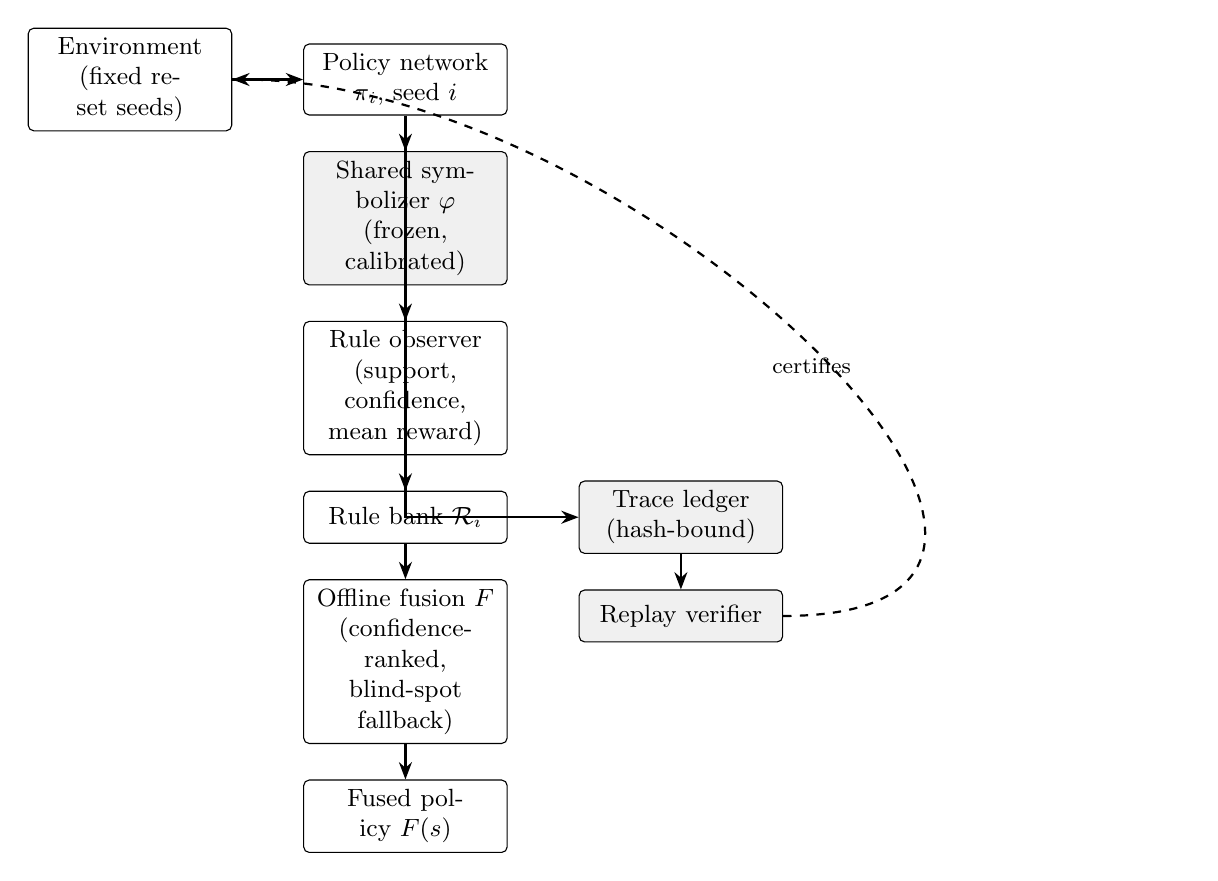
\begin{tikzpicture}[
  node distance=0.45cm and 0.9cm,
  box/.style={draw, rounded corners=2pt, align=center, minimum height=0.66cm, font=\small, fill=white, text width=2.35cm},
  arrow/.style={-{Stealth[length=2.2mm]}, thick},
  dim/.style={fill=black!6}
]
\node[box] (env) {Environment\\ (fixed reset seeds)};
\node[box, right=of env] (actor) {Policy network\\ $\pi_i$, seed $i$};
\node[box, dim, below=of actor] (sym) {Shared symbolizer $\varphi$\\ (frozen, calibrated)};
\node[box, below=of sym] (obs) {Rule observer\\ (support, confidence, mean reward)};
\node[box, below=of obs] (bank) {Rule bank $\mathcal{R}_i$};
\node[box, below=of bank] (fusion) {Offline fusion $F$\\ (confidence-ranked,\\ blind-spot fallback)};
\node[box, below=of fusion] (policy) {Fused policy $F(s)$};
\node[box, dim, right=of bank] (ledger) {Trace ledger\\ (hash-bound)};
\node[box, dim, below=of ledger] (replay) {Replay verifier};

\draw[arrow] (env) -- (actor);
\draw[arrow] (actor) -- (sym);
\draw[arrow] (sym) -- (obs);
\draw[arrow] (obs) -- (bank);
\draw[arrow] (bank) -- (fusion);
\draw[arrow] (fusion) -- (policy);
\draw[arrow] (actor.south) |- (ledger.west);
\draw[arrow] (ledger) -- (replay);
\draw[arrow,dashed] (replay.east) to[out=0,in=0,looseness=1.35] node[below,pos=0.5,font=\footnotesize]{certifies} (env.east);
\end{tikzpicture}
\caption{The auditable rule-induction protocol. A frozen shared symbolizer makes rule banks
comparable across seeds; a hash-bound ledger and replay verifier certify fidelity; offline fusion
composes rule banks into a single auditable policy. Dashed edge: the replay verifier re-executes
the recorded actions in the environment under the recorded reset seeds.}
\label{fig:pipeline}
\end{figure}

\subsection{Shared state symbolizer}
\label{sec:method:symbolizer}

All agents operate on the same continuous state space, but independently trained networks may rely
on different parts of it. To make descriptions comparable, we fix \emph{one} symbolizer before any
agent is trained and freeze it. For each state dimension $j\in\{1,\ldots,d\}$, pooled empirical
quantiles are computed from separate random-policy roll-ins (24 episodes per seed), yielding three
cut points per dimension and four bins. The symbolizer is
\begin{equation}
\varphi(s) \;=\; \big(\,\mathrm{bin}_1(s_1),\ldots,\mathrm{bin}_d(s_d)\big)\;\in\;\{0,1,2,3\}^{d},
\label{eq:symbolizer}
\end{equation}
so the shared vocabulary has $4^{d}$ symbols ($256$ symbols for CartPole-v1, $4096$ for
Acrobot-v1). The quantiles are computed once and never updated, so every seed and every arm of the
experiment sees the same abstraction. This design choice is coupled to everything downstream; we
discuss its alternatives in Section~\ref{sec:discussion}.

\subsection{Rule bank and admission}
\label{sec:method:rules}

A \emph{rule} is a pair $(\mathbf{c},a)$ where $\mathbf{c}=\varphi(s)$ is a condition (a discrete
state symbol) and $a\in\mathcal{A}$ is an action. From the logged trace of agent $i$, the observer
computes, for every condition--action pair,
\begin{equation}
n_{\mathbf{c},a} \;=\; \#\{(s,a)\in \mathcal{T}_i : \varphi(s)=\mathbf{c}\},
\qquad
f_{\mathbf{c},a} \;=\; \frac{n_{\mathbf{c},a}}{\sum_{a'} n_{\mathbf{c},a'}},
\qquad
\mu_{\mathbf{c},a} \;=\; \frac{1}{n_{\mathbf{c},a}}\sum_{r\in \mathcal{T}_i(\mathbf{c},a)} r,
\label{eq:rulestats}
\end{equation}
where $\mathcal{T}_i$ is the transition set of agent $i$ and $r$ is the immediate reward. The
condition--action pair is admitted into the rule bank $\mathcal{R}_i$ if and only if
\begin{equation}
\mathrm{Adm}(\mathbf{c},a)\;\equiv\;\big(n_{\mathbf{c},a}\ge \tau_{s}\big)\ \wedge\ \big(f_{\mathbf{c},a}\ge \tau_{c}\big),
\qquad \tau_{s}=8,\ \tau_{c}=0.70 .
\label{eq:admission}
\end{equation}
We call $f_{\mathbf{c},a}$ the \emph{confidence} of the rule. The admission predicate is a
deterministic reduction of the trace: it compresses logged statistics without sampling, so its
output is exactly reproducible from the same trace.

\subsection{Audit ledger and replay verification}
\label{sec:method:ledger}

Fidelity is certified by two independent mechanisms.

\emph{Environment replay.} For every recorded transition, the verifier re-executes the environment
under the recorded reset seed with the recorded action and compares the resulting state, reward,
termination, and truncation flags against the recorded values:
\begin{equation}
\mathrm{Replay}\big((s,a,r,s',\mathrm{term},\mathrm{trunc});\,k\big)\ \equiv\ \big[\mathrm{Env}(s,a;k) = (s',r,\mathrm{term},\mathrm{trunc})\big],
\label{eq:replay}
\end{equation}
where $\mathrm{Env}(\cdot;k)$ is the deterministic environment transition under reset seed $k$ and
equality is exact float32 equality. Replay is a transport-level check: it certifies that the logged
trace is the executed trace, and it says nothing about whether the policy is good.

\emph{Hash-bound ledger.} Every training event (environment transition and optimizer update) is
serialized into a canonical payload and appended to a hash chain
\begin{equation}
h_0 = H(\mathrm{init}), \qquad h_{t} = H\big(h_{t-1} \,\Vert\, \mathrm{payload}_t\big),
\label{eq:hashchain}
\end{equation}
with SHA-256. The chain is recomputed from the raw payloads and compared against the recorded chain;
a mismatch at any position invalidates the entire run. An update ledger records, for each optimizer
step, the checkpoint hash before and after the step, so the chain certifies the sequence of weight
states as well as the sequence of transitions.

\subsection{Training arms}
\label{sec:method:arms}

Each seed trains three arms with identical hyperparameters and reset seeds:
\begin{itemize}
  \item \emph{Baseline:} unconstrained REINFORCE.
  \item \emph{Audit-only observer:} identical to the baseline (same weights, same trace hash) but the
        rule observer runs alongside and emits a rule bank from the training trace. Its actor is
        byte-identical to the baseline actor, which we verify explicitly.
  \item \emph{Constrained:} the action distribution is masked so that only actions admitted by rules
        extracted from the agent's own earlier trace can be selected during training.
\end{itemize}
The constrained arm was part of the original design intuition (\emph{let the rules steer the
training}) and is retained in the experiment to quantify the cost of that intuition
(Section~\ref{sec:evolution:constraint}).

\subsection{Rule-level policy fusion}
\label{sec:method:fusion}

Given rule banks $\{\mathcal{R}_i\}_{i=1}^{n}$ from $n$ seeds, the fused policy makes a decision at
state $s$ as follows (Figure~\ref{alg:fusion}). Let
$\mathcal{C}(s)=\{\,r\in\textstyle\bigcup_i \mathcal{R}_i : \mathbf{c}_r=\varphi(s)\,\}$ be the set of
candidate rules whose condition matches the current state. If $\mathcal{C}(s)=\varnothing$, the
state is a \emph{blind spot} and the fused policy falls back to the action of a fixed single actor
selected by its training return (the actor-logit argmax). Otherwise, the fused action is the action
of the candidate with the highest confidence; ties are broken by support, then by mean reward, then
by source index. Formally,
\begin{equation}
F(s) \;=\; \begin{cases}
\displaystyle \arg\max_{a}\,\max_{r\in\mathcal{C}(s)} w(r)\,\mathbf{1}[a_r=a], & \mathcal{C}(s)\neq\varnothing,\\[2mm]
\pi_{\mathrm{fb}}(s), & \mathcal{C}(s)=\varnothing,
\end{cases}
\label{eq:fusion}
\end{equation}
where $w(r)=(f_r,\ n_r,\ \mu_r,\ -i)$ in lexicographic order and $\pi_{\mathrm{fb}}$ is the fallback
actor. Two per-decision quantities are recorded for every step:
\begin{equation}
\mathrm{cov}(s)=\mathbf{1}[\mathcal{C}(s)\neq\varnothing], \qquad
\mathrm{confl}(s)=\mathbf{1}\big[\#\{a_r : r\in\mathcal{C}(s)\}>1\big].
\label{eq:coverage}
\end{equation}
We call $\mathrm{confl}(s)=1$ a \emph{conflict}: the seeds disagree about the action for this
condition.

\begin{figure}[t]
\centering
\caption{Rule-level policy fusion.}
\label{alg:fusion}
\begin{minipage}{0.88\textwidth}
\small
\textbf{Input:} rule banks $\mathcal{R}_1,\ldots,\mathcal{R}_n$; symbolizer $\varphi$; fallback actor $\pi_{\mathrm{fb}}$.
\vspace{0.35em}

For each decision at state $s$:
\begin{enumerate}
  \item $\mathbf{c}\leftarrow \varphi(s)$
  \item $\mathcal{C}\leftarrow\{\,r\in\bigcup_i\mathcal{R}_i : \mathbf{c}_r=\mathbf{c}\,\}$ \hfill (candidate rules)
  \item \textbf{if} $\mathcal{C}=\varnothing$ \textbf{then return} $\pi_{\mathrm{fb}}(s)$ \hfill (blind spot: fallback)
  \item $r^{*}\leftarrow \arg\max_{r\in\mathcal{C}}\ (f_r,\ n_r,\ \mu_r,\ -i)$ \hfill (lexicographic order)
  \item \textbf{return} $a_{r^{*}}$
\end{enumerate}
\end{minipage}
\end{figure}

\subsection{Analysis instruments}
\label{sec:method:instruments}

Three instruments probe what the rules and the fused policy actually mean.

\emph{Behavioral agreement.} For two actors $\pi_i,\pi_j$, sample $N$ fresh states from each
actor's own occupancy and measure the proportion on which the two policies select the same action:
\begin{equation}
\bar{A}(\pi_i,\pi_j) \;=\; \frac{1}{N}\sum_{s\in\mathcal{S}_{ij}} \mathbf{1}[\pi_i(s)=\pi_j(s)],
\label{eq:agreement}
\end{equation}
where $\mathcal{S}_{ij}$ is the pooled fresh-state sample. Because the states are drawn by
occupancy rather than uniformly, we also report an episode-cluster-balanced estimate and a
cluster-balanced bootstrap interval.

\emph{Rule-set overlap.} Rule banks are compared with the Jaccard similarity of their exact
state--action sets,
\begin{equation}
J(\mathcal{R}_i,\mathcal{R}_j) \;=\; \frac{\lvert \mathcal{R}_i \cap \mathcal{R}_j \rvert}{\lvert \mathcal{R}_i \cup \mathcal{R}_j \rvert},
\label{eq:jaccard}
\end{equation}
together with the number of shared conditions whose recommended actions conflict.

\emph{Fitted-Q GPI baseline.} To place the fusion comparison on a principled footing, we fit, for
each frozen source actor $\pi_i$, an action-value regressor by fitted Q evaluation (FQE)
\cite{le2019batch,voloshin2021empirical} over a pooled replay buffer:
\begin{equation}
\hat{Q}^{(k+1)}(s,a) \;=\; r + \gamma\,\hat{Q}^{(k)}\big(s',\,\arg\max\nolimits_{a'}\pi_i(s')\big),
\label{eq:fqe}
\end{equation}
minimized in the least-squares sense over the replay transitions, with a reservoir cap of 25,000
transitions per seed and $\gamma=0.99$. The baseline policy is the generalized policy improvement
(GPI) selection \cite{sutton2018reinforcement}
\begin{equation}
\pi_{\mathrm{GPI}}(s) \;=\; \arg\max_{a}\,\max_{i}\,\hat{Q}_i(s,a).
\label{eq:gpi}
\end{equation}
We emphasize that this is an \emph{approximate} GPI: the classical GPI bound requires bounded value
estimation error, which we do not claim to control; the fitted critics are diagnostics, and their
failure is informative but not evidence about exact GPI.

\subsection{Statistical conventions}
\label{sec:method:stats}

All composition evaluations use 100 held-out episodes per policy, with reset seeds
$20{,}000{,}000 + i$ for $i=0,\ldots,99$; every policy sees the same episodes, so policy comparisons
are paired at the episode level. Paired differences are summarized by the mean of the per-episode
difference, with a 95\% percentile bootstrap interval over episodes (10{,}000 resamples). Standard
deviations are cross-episode sample standard deviations; we do not claim cross-seed variance
estimates, because the seed pool ($n=8$) is too small for that purpose. Where a quantity is
deterministic (replay equality, hash validity), we state that variance is structurally zero.

% ----------------------------------------------------------------------
\section{From Intuition to Protocol: a Failure-Driven Design History}
\label{sec:evolution}

This section documents, in order, the failures that shaped the protocol. Each entry states the
failure, its cause, and the change it forced. The sequence is part of the scientific record: it
explains why the protocol looks the way it does, and it is evidence about which intuitions are
unsafe.

\subsection{Why replay is not explanation}
\label{sec:evolution:replay}

The first intuition is that a recorded trace \emph{is} the explanation: ``here is exactly what the
agent did.'' A trace is faithful, but it is not a description. A full trace of a single seed on
CartPole-v1 contains $\approx$97{,}646 transitions (and up to 300{,}000 records per arm across the
population); a human cannot inspect it, two traces cannot be compared except by exact matching, and
a trace says nothing about states the agent never visited. The lesson, formalized as
Section~\ref{sec:method:ledger}, is that traces belong to the fidelity layer, and a separate
compression step is needed for the description layer. We therefore treat \emph{trace} and
\emph{rule bank} as distinct artifacts with distinct evidentiary roles.

\subsection{First-generation prototype failures}
\label{sec:evolution:v1}

An initial prototype attempted to compress behavior with sequence grammar induction. Three defects
were found, each independently fatal for the intended claim:

\begin{enumerate}
  \item \emph{Lossy grammar.} The prototype's sequence-compression inducer was a simplified variant
        of SEQUITUR \cite{nevillmanning1997identifying} and was not equivalent to the published
        algorithm. The induced grammar could not be proven to reproduce the source sequence, so any
        rule extracted from it was not anchored to the trace. Cause: reimplementing a linear-time
        grammar algorithm from memory without a conformance test. Fix: discard grammar-based
        compression as an evidence path; compress only \emph{statistics} (support, confidence, mean
        reward) whose computation is a deterministic reduction of the trace.
  \item \emph{Conflation of one-step and window rules.} The observer initially treated ``the agent
        chose $a$ in condition $\mathbf{c}$'' and ``the agent repeated a pattern across several
        steps'' as the same kind of rule. They are different quantities: the first is a per-decision
        statistic, the second a sequence property. Mixing them produced rules with no well-defined
        estimand. Cause: one object was used for two jobs. Fix: the protocol admits only per-decision
        condition--action rules (\ref{eq:rulestats}); sequence structure is outside the evidence
        budget of this paper.
  \item \emph{``Replay'' meant different things.} An early verifier checked that recorded actions,
        when replayed, reproduced \emph{some} transition statistics; it did not check exact
        per-transition equality. Cause: the verifier tested aggregate health, not fidelity. Fix:
        exact float32 equality per transition (\ref{eq:replay}), replayed from the recorded reset
        seed.
\end{enumerate}

\subsection{Rule-constrained training damages behavior}
\label{sec:evolution:constraint}

The original design intuition was that induced rules should actively guide training: mask out
actions that violate the agent's own rules. A pilot run showed a catastrophic effect: the
constrained actor's held-out return fell from 500 (the environment ceiling) to 121.3, and rule
coverage during training collapsed to 0.4\% of steps. The full eight-seed study confirms the
heterogeneity (Table~\ref{tab:perseed}): on CartPole-v1, constraining training improved some seeds
(29: 131.0$\rightarrow$293.5; 71: 130.2$\rightarrow$387.2; 43: 153.8$\rightarrow$500.0) but
destroyed others (11: 500.0$\rightarrow$182.3; 149: 500.0$\rightarrow$96.1; 307:
500.0$\rightarrow$161.2). On Acrobot-v1 every seed's held-out return is $-500$ in both arms.

The cause is structural. The rule mask changes the data distribution: actions that the mask prunes
are never executed, so their conditions receive no new support, coverage shrinks, and the policy is
steered into a shrinking subset of the state space. The same rule machinery that \emph{composes}
well offline (Section~\ref{sec:experiments:cartpole}) is unsafe as a training-time intervention.
Consequence: the protocol separates rule induction (audit-only observer) from rule composition
(offline fusion); the constrained arm is retained only as a quantified negative result.

\begin{table}[t]
\centering
\caption{Per-seed held-out returns on CartPole-v1 (100 common reset seeds): baseline actor versus
the rule-constrained actor. The constraint is a training-time intervention; its effect is
heterogeneous and is negative for every seed that reaches the ceiling without it. On Acrobot-v1
every seed returns $-500$ in both arms.}
\label{tab:perseed}
\begin{tabular}{lccc}
\toprule
Seed & Baseline & Constrained & Change \\
\midrule
11 & 500.0 & 182.3 & $-317.7$ \\
29 & 131.0 & 293.5 & $+162.5$ \\
43 & 153.8 & 500.0 & $+346.3$ \\
71 & 130.2 & 387.2 & $+257.0$ \\
101 & 201.3 & 149.2 & $-52.2$ \\
149 & 500.0 & 96.1 & $-403.9$ \\
211 & 500.0 & 403.2 & $-96.8$ \\
307 & 500.0 & 161.2 & $-338.8$ \\
\bottomrule
\end{tabular}
\end{table}

\subsection{Confidence thresholds and the 100\% blind-spot collapse}
\label{sec:evolution:threshold}

Rule admission requires a confidence threshold. A high-confidence variant ($\tau_c=0.90$) produced
fusion policies that deferred to the fallback actor on 100\% of held-out decisions: the strict
threshold admitted so few rules that no condition was covered, and the ``fusion'' was the fallback
in disguise. Cause: confidence is a conditional statistic; raising it shrinks support monotonically,
and at the extreme the rule bank no longer covers the state space. The threshold was therefore set
to $\tau_c=0.70$ with $\tau_s=8$ \emph{and} an explicit blind-spot fallback (\ref{eq:fusion}) so
that coverage failure is observable rather than silent. This is a two-setting exploratory choice,
not a systematic threshold search; we report the boundary in
Section~\ref{sec:experiments}.

\subsection{Serialization and ledger-schema failures}
\label{sec:evolution:serialization}

Two failures concerned the audit artifacts themselves. First, a human-readable (pretty-printed)
serialization of the trace inflated its size by roughly $1.8\times$; after switching to a compact
canonical encoding, the compressed trace ledger was still 8.4\% larger (CartPole-v1) and 9.9\%
larger (Acrobot-v1) than the gzip-compressed raw trace, because the grammar-style codec adds
structure without removing bytes. The codec is nevertheless exact: the decoded payload hashes to the
input hash. We report these costs as part of practical reproducibility. Second, the update-ledger
schema initially allowed a sidecar field (a grammar-generation annotation) to vary without changing
the optimizer record, so two runs with identical optimizer behavior could hash differently.
Cause: the hash covered non-core fields. Fix: the ledger hashes only a normalized core record
(step index, parameter gradient hash, pre/post checkpoint hashes), making equivalent runs hash
identically.

% ----------------------------------------------------------------------
\section{Experiments and Results}
\label{sec:experiments}

\subsection{Setup}
\label{sec:experiments:setup}

Experiments use CartPole-v1 (4 state dimensions, 2 actions) and Acrobot-v1 (6 dimensions, 3
actions) from the Gymnasium suite \cite{towers2024gymnasium}. Eight seeds
$\{11,29,43,71,101,149,211,307\}$ are used; each seed trains 300 episodes per arm with REINFORCE
(\ref{eq:reinforce}) and a shared frozen symbolizer (\ref{eq:symbolizer}) calibrated from 24
random-policy episodes per seed. Rules are admitted with $(\tau_s,\tau_c)=(8,0.70)$. Composition
evaluates 100 held-out episodes per policy on the common reset seeds. All reported traces were
post-hoc audited: hash chains, update ledgers, baseline/observer equivalence, and environment
replay were re-verified after the runs completed.

\subsection{Audit integrity}
\label{sec:experiments:integrity}

Table~\ref{tab:integrity} reports the fidelity layer. Every hash chain is valid, every update
ledger verifies, baseline and audit-only actors are byte-identical, and every recorded transition
replays exactly under its reset seed. The lossless codec round-trips exactly in both environments.
These are operational-health results: they certify the artifacts, and they do not by themselves
support any claim about policy quality.

\begin{table}[t]
\centering
\caption{Audit integrity (operational-health layer). Values are deterministic; variance is
structurally zero.}
\label{tab:integrity}
\begin{tabular}{lcc}
\toprule
 & CartPole-v1 & Acrobot-v1 \\
\midrule
Trace records (all three arms) & 1{,}725{,}655 & 2{,}544{,}513 \\
Optimizer update records & 7{,}200 & 7{,}200 \\
Environment replay checks (post-hoc) & 1{,}122{,}403 & 1{,}742{,}570 \\
Constraint rule-reference verifications & 290{,}052 & 697{,}817 \\
Hash chains valid & yes & yes \\
Update ledgers valid & yes & yes \\
Baseline vs.\ audit-only actor identical & yes & yes \\
Codec round-trip exact & yes & yes \\
Raw trace bytes / gzip & 61.3\,MB / 12.3\,MB & 57.6\,MB / 12.5\,MB \\
Codec archive (gzip) & 13.4\,MB & 13.7\,MB \\
\bottomrule
\end{tabular}
\end{table}

\subsection{Rule structure across seeds}
\label{sec:experiments:structure}

Rule banks are seed-specific but structurally related (Table~\ref{tab:structure}). On CartPole-v1,
all eight seeds share a core of 38 conditions on which they \emph{agree} (same action in every
seed), and the mean pairwise Jaccard overlap of rule sets is 0.56; the two-seed comparison used
throughout the report is 0.58. On Acrobot-v1 the picture inverts: the all-seed intersection contains
only 2 conditions, and both are \emph{conflicting}; the mean pairwise Jaccard is 0.096. Across the
two environments, 77 of 98 shared conditions conflict in Acrobot-v1 versus 0 of 77 in CartPole-v1.

\begin{table}[t]
\centering
\caption{Rule structure across seeds. Pairwise statistics use all 28 seed pairs.}
\label{tab:structure}
\begin{tabular}{lcc}
\toprule
 & CartPole-v1 & Acrobot-v1 \\
\midrule
Rule count per seed (range) & 100--145 & 77--303 \\
Conditions shared by $\ge$2 seeds & 165 & 445 \\
All-seed intersection (conditions) & 38 & 2 \\
\quad same-action core & 38 & 0 \\
\quad conflicting & 0 & 2 \\
Mean pairwise rule Jaccard (\ref{eq:jaccard}) & 0.557 & 0.096 \\
Shared conditions (seeds 11 vs.\ 29) & 77 & 98 \\
\quad conflicting (seeds 11 vs.\ 29) & 0 & 77 \\
\bottomrule
\end{tabular}
\end{table}

\subsection{Composition on CartPole-v1}
\label{sec:experiments:cartpole}

Table~\ref{tab:primary} and Figure~\ref{fig:cartpole} report the main composition result. On
CartPole-v1, the rule-level fusion policy reaches a mean held-out return of 205.96 (median 181,
cross-episode std 79.1) versus 163.65 for the best single actor, a paired difference of $+42.31$
with 95\% bootstrap interval $[23.98,61.93]$. Fusion decisions are 98.3\% rule-covered (20{,}240 of
20{,}596 steps) with only 75 conflicting decisions (0.4\%) and 356 blind spots (1.7\%), which is
consistent with the low-conflict rule structure of Table~\ref{tab:structure}. The actor-logit
ensemble saturates the environment ceiling (500.0, zero variance), which makes it a ceiling-level
comparison rather than a differentiating one.

\begin{table}[t]
\centering
\caption{Primary composition results. Means and paired differences over 100 common held-out
episodes; 95\% bootstrap intervals in brackets.}
\label{tab:primary}
\begin{tabular}{lcc}
\toprule
Policy & CartPole-v1 & Acrobot-v1 \\
\midrule
Best single actor & 163.65 & $-500.0$ \\
Actor-logit ensemble & 500.0 (ceiling) & $-500.0$ \\
Grammar fusion $F$ (\ref{eq:fusion}) & \textbf{205.96} & $-443.37$ \\
Fitted-Q GPI (\ref{eq:gpi}) & 9.34 & $-499.57$ \\
\midrule
Paired $\Delta$ fusion vs.\ best single & $+42.31\ [23.98,\,61.93]$ & $+56.63\ [39.32,\,75.15]$ \\
Paired $\Delta$ ensemble vs.\ best single & $+336.35$ & $0.0$ \\
Fusion coverage / conflicts / blind spots & 98.3\% / 75 / 356 & 95.7\% / 39{,}602 / 1{,}909 \\
\bottomrule
\end{tabular}
\end{table}

\begin{figure}[t]
\centering

\includegraphics[width=0.72\textwidth]{paper_figs/fig_cartpole_composition.pdf}
\caption{CartPole-v1 composition comparison. Error bars are 95\% bootstrap intervals of the mean
over the 100 held-out episodes. The dashed line marks the environment ceiling (500). The
actor-logit ensemble and the FQE-GPI baseline bracket the fusion result from above and below;
FQE-GPI is reported here and analyzed as a failed diagnostic in
Section~\ref{sec:experiments:fqe}.}
\label{fig:cartpole}
\end{figure}

\subsection{Acrobot-v1: the conflict regime and the failure of confidence arbitration}
\label{sec:experiments:acrobot}

On Acrobot-v1, every source actor is at the floor ($-500$), yet the fusion policy is not: it
averages $-443.37$ (median $-500$, std 90.8), with 39 of 100 episodes terminating before the
500-step cap and a maximum of $-126$. The paired difference versus the best single actor is $+56.63$
$[39.32,75.15]$. However, the fusion decisions are 95.7\% rule-covered and 89.2\% \emph{conflicting}
(39{,}602 of 44{,}376 steps), so the fused policy is almost entirely an arbitration among
disagreeing seeds.

The arbitration rule matters enormously, and not in the intended direction
(Figure~\ref{fig:acrobot}, Table~\ref{tab:ablations}). Uniformly random arbitration among candidate
rules returns $-187.02$ on the primary evaluation (95\% paired interval $[231.38,278.21]$ relative
to confidence-ranked fusion) and is replicated across five independent random-number streams with
means from $-206.17$ to $-194.10$ (overall $-198.82$). By contrast, confidence-ranked arbitration
returns $-443.37$; mean-reward-first, support-first, defer-to-ensemble, and unanimous-only
arbitration all return $-500$; and the single-source fallbacks return $-499.5$ and $-500$. A matched
control that ignores the rules entirely and samples uniformly random actions averages $-498.71$
across five replicates. Confidence-ranked arbitration is therefore not merely suboptimal but
\emph{anti-selective}: on this task, choosing rules by confidence selects worse actions than
choosing them at random.

A 200-state Monte-Carlo action-semantics probe (fresh states from deterministic actor rollouts)
dissects the failure (Table~\ref{tab:mcprobe}). The fusion policy covers all 200 states, conflicts
on 90.5\% of them, and agrees with the best first action (counterfactual continuation return under
the actor-logit ensemble) on only 22.5\% of states; its action histogram also differs sharply from
the Monte-Carlo-optimal histogram. The mean margin between the best and second-best first actions is
108.2 return units, so the decisions are not near-ties. The confidence signal that arbitration
relies on does not track the Monte-Carlo ranking of first actions in this environment.

\begin{table}[t]
\centering
\caption{Acrobot-v1: arbitration ablations on the 100 matched held-out episodes. Paired intervals
are bootstrap 95\% intervals of the per-episode difference relative to the current
confidence-ranked policy.}
\label{tab:ablations}
\begin{tabular}{lcc}
\toprule
Arbitration rule & Mean return & Paired 95\% interval vs.\ current \\
\midrule
Confidence-first (current) & $-443.37$ & --- \\
Confidence only (no tie-breaks) & $-444.49$ & $[-3.16,\ 0.06]$ \\
Random candidate & $-187.02$ & $[231.38,\ 278.21]$ \\
Mean reward first & $-500.0$ & $[-75.47,\ -39.67]$ \\
Support first & $-500.0$ & $[-74.84,\ -39.68]$ \\
Defer conflicts to ensemble & $-500.0$ & $[-75.12,\ -40.08]$ \\
Unanimous only & $-500.0$ & $[-74.49,\ -39.36]$ \\
Best single fallback & $-452.69$ & $[-19.51,\ 0.50]$ \\
Single source 11 / 29 & $-499.48$ / $-500.0$ & --- \\
\bottomrule
\end{tabular}
\end{table}

\begin{figure}[t]
\centering

\includegraphics[width=0.72\textwidth]{paper_figs/fig_acrobot_ablations.pdf}
\caption{Acrobot-v1 arbitration ablations on matched episodes. Random arbitration among candidate
rules (solid red bar) substantially outperforms confidence-ranked arbitration; the dashed line marks
the five-stream random-arbitration mean. Uniform random actions (ignoring the rules) average
$-498.71$ and are omitted for scale.}
\label{fig:acrobot}
\end{figure}

\begin{table}[t]
\centering
\caption{Acrobot-v1 Monte-Carlo action-semantics probe on 200 fresh states (state sample from new
deterministic actor rollouts). ``Best first action'' is the action maximizing counterfactual
continuation return when followed by the actor-logit ensemble.}
\label{tab:mcprobe}
\begin{tabular}{lc}
\toprule
Quantity & Value \\
\midrule
Fusion coverage & 100\% \\
Fusion conflict rate & 90.5\% \\
Fusion agreement with any source-$Q$ argmax & 64.5\% \\
Fusion agreement with ensemble-GPI argmax & 0.0\% \\
\textbf{Fusion agreement with MC-best first action} & \textbf{22.5\%} \\
MC continuation return, first action 0 / 1 / 2 & $-132.9$ / $-202.5$ / $-157.1$ \\
MC-best first-action histogram (0/1/2) & 87 / 46 / 67 \\
Mean best-vs-second margin & 108.2 \\
\bottomrule
\end{tabular}
\end{table}

\subsection{Behavioral agreement: rule overlap does not transfer}
\label{sec:experiments:agreement}

Rule-set overlap and behavioral agreement measure different things, and the data show how different
they are (Figure~\ref{fig:agreement}). On CartPole-v1, the rule banks of seeds 11 and 29 share a
Jaccard overlap of 0.58 and agree on all 77 shared conditions, and the mean pairwise rule overlap
is 0.56. Yet on 10{,}000 fresh states (5{,}000 from each actor's own occupancy), the two policies
select the same action on only 51.4\% of states (episode-cluster-balanced estimate 51.4\%; 95\%
bootstrap interval $[50.5,52.3]$). Within each actor's own occupancy the agreement is 50.6\% and
52.2\% respectively. Stratifying by pole angle shows the agreement is near chance for near-zero
angles (50.2\%) and only modestly above chance in the mid range (55.8\%). The rules of these two
agents overlap almost completely, yet the agents behave almost independently on fresh states.
Rule-set overlap is therefore not a proxy for behavioral agreement; it is an upper-layer statistic
that must be validated against the behavior itself.

\begin{figure}[t]
\centering

\includegraphics[width=0.72\textwidth]{paper_figs/fig_agreement.pdf}
\caption{CartPole-v1: rule-set overlap (Jaccard, seeds 11 vs.\ 29 and all 28 pairs) versus
behavioral agreement on 10{,}000 fresh states. Error bar: 95\% bootstrap interval of the
cluster-balanced agreement. The dashed line marks chance (0.5).}
\label{fig:agreement}
\end{figure}

\subsection{Fitted-Q GPI baseline failure}
\label{sec:experiments:fqe}

The fitted-Q GPI baseline (\ref{eq:fqe}--\ref{eq:gpi}) fails in both environments, and the failure
mode is informative. On CartPole-v1 its mean return is 9.34 (paired difference $-154.31$ versus the
best single actor), and the fitted critics are nearly flat: the critic values have cross-seed
agreement of 0.84 on greedy actions but their pointwise standard deviation is only 0.81 around a
mean of 10.7, i.e., the $Q$-estimates carry almost no signal across states. The FQE-GPI action
histogram is 30{,}758:805 (nearly always action 0), and its agreement with the actor-logit ensemble
on 31{,}563 held-out states is 35.3\%. On Acrobot-v1 the collapse is total: FQE-GPI selects action 0
on all 50{,}000 held-out states, the critics are constant at $-11.44$ with standard deviation
0.009, greedy-action agreement between critics is 6.3\%, and the held-out Bellman residual is 0.92
(MAE), which is far from the precision that the GPI bound would require. These are diagnostics, not
discoveries: they show that fitted-Q composition over a 200k-transition reservoir is unreliable in
these setups, and they caution against claiming that the rule-fusion result is ``better than
value-based composition'' on the strength of this baseline alone.

\subsection{Summary of verdicts}
\label{sec:experiments:verdicts}

\begin{table}[t]
\centering
\caption{Summary of measurement layers. Identification-bearing results are distinguished from
diagnostics and operational-health checks.}
\label{tab:verdicts}
\begin{tabular}{llcc}
\toprule
Criterion & Layer & CartPole-v1 & Acrobot-v1 \\
\midrule
Trace/hash/replay validity & operational health & pass & pass \\
Rule overlap across seeds & diagnostic & 0.557 & 0.096 \\
Fusion vs.\ best single (paired $\Delta$) & measured, capped & $+42.31$ & $+56.63$ \\
Fusion mean return & measured & 205.96 & $-443.37$ \\
Random arbitration vs.\ confidence & identification & n/a & $-187.02$ vs.\ $-443.37$ \\
Behavioral agreement (fresh states) & identification & 51.4\% ($\approx$ chance) & n/a \\
FQE-GPI mean return & diagnostic & 9.34 & $-499.57$ \\
\bottomrule
\end{tabular}
\end{table}

Table~\ref{tab:verdicts} separates the layers. The identification-bearing findings are (i) the
paired fusion advantage on CartPole-v1, (ii) the behavioral-agreement near-chance result, and
(iii) the Acrobot arbitration reversal. All other rows are diagnostics or health checks.

% ----------------------------------------------------------------------
\section{Related Work}
\label{sec:related}

\emph{Policy description and interpretability of RL.} Post-hoc interpretability of policies
typically produces saliency or attribution maps rather than inspectable behavioral rules, and such
maps do not certify behavior on unseen states. Rule extraction for RL has a long line of work using
decision trees and program synthesis; the present study differs in that rules are induced from a
\emph{shared, frozen symbolizer} so that rule banks from different seeds are directly comparable,
and in that every rule is anchored to a replayed, hash-bound trace.

\emph{Value-based composition.} Policy improvement theorems \cite{sutton2018reinforcement} show how
a value function can certify improvement over a base policy, and generalized policy improvement
combines several value functions. Those guarantees require accurate value estimates. Our fitted-Q
GPI baseline (\ref{eq:gpi}) fails precisely because the fitted critics are nearly constant, which
is a failure mode documented for FQE under off-policy coverage limits
\cite{le2019batch,voloshin2021empirical}. We do not position rule fusion as a replacement for
value-based composition; the evidence supports only the bounded claim that, under a shared
symbolizer, rule-level arbitration can exceed the best single actor in a low-conflict regime.

\emph{Discrete symbolic communication and auditability.} The ``AI Mother Tongue'' line of work
shows that VQ-VAE-derived discrete symbols can serve as an endogenous communication channel between
agents \cite{liu2025aim}, and its audit agenda asks whether coordination logic can be reconstructed
from discrete symbol logs without hidden channels. The present work shares the audit agenda but
does not rely on emergent communication: our symbols are a fixed calibration-derived abstraction,
not a learned codebook, so the two lines are complementary rather than competing. We do not claim
any result about learned symbol systems.

\emph{Auditability of training records.} Ledgering and replay verification of training runs are
reproducibility practices. Our contribution on this axis is limited but explicit: a hash-bound
ledger over canonical payloads plus exact environment replay, with the negative findings that
human-readable serialization inflates size and that grammar-style codecs can fail to compress
traces. These are practical reproducibility findings, not new cryptography.

% ----------------------------------------------------------------------
\section{Discussion}
\label{sec:discussion}

\subsection{Why the mechanism may work, and where it breaks}
\label{sec:discussion:mechanism}

The CartPole advantage of rule-level fusion has a simple account in the equations. The fused
decision (\ref{eq:fusion}) selects the highest-confidence rule among the candidates
(\ref{eq:admission}); when conflicts are rare (0 of 77 shared conditions), the fused policy is
essentially a union of the seeds' agreement, and the fallback (\ref{eq:fusion}, second case) covers
the residual 1.7\% of states. The paired comparison controls for the reset-seed distribution, and
the bootstrap interval excludes zero. But the same equations fail on Acrobot-v1 because the
confidence statistic $f_{\mathbf{c},a}$ (\ref{eq:rulestats}) is a \emph{within-trace} conditional
frequency, not a predictor of which action is best in a new state: when 89\% of decisions conflict
and the best first action (probe, Table~\ref{tab:mcprobe}) disagrees with the fused choice on
77.5\% of states, the arbitration is selecting on a signal that does not rank actions by return.
The reversal---random arbitration beating confidence arbitration---is consistent with the
Monte-Carlo probe: the confidence-ranked action is anti-correlated with the best first action in
this regime, so removing the signal helps. We state this as an \emph{open mechanism}: we can show
the signal is uninformative, but we cannot yet explain why it is \emph{negatively} informative on
Acrobot-v1.

\subsection{Prediction outcomes}
\label{sec:discussion:predictions}

Two expectations held and two failed. Expected: (i) trace fidelity (replay, hashes) would verify
cleanly, and (ii) rule overlap would be higher under a shared symbolizer than under per-seed
symbolizers (the design motivation). Unexpected: (iii) behavioral agreement would track rule
overlap---it does not (51.4\% vs.\ chance), and (iv) confidence-ranked arbitration would dominate
random arbitration---it is reversed on Acrobot-v1. For (iii), an alternative explanation is that
the shared symbolizer is too coarse: with only four bins per dimension, two policies can agree on
rules for the symbol while disagreeing on nearly every state inside the symbol; the rules describe
the \emph{symbol}, and behavior lives on \emph{states}. For (iv), an alternative explanation is
that the trace's confidence is dominated by the early, poorly-performing part of training in
Acrobot-v1 (where all returns are $-500$ and mean reward is constant at $-1.0$ for 93\% of rules),
so confidence reflects state-visitation frequency rather than action quality. Both alternatives are
testable and are the natural next experiments.

\subsection{Theoretical and practical implications}
\label{sec:discussion:implications}

Theoretical implication: under a shared, frozen symbolizer, rule-level composition inherits
provable properties only for the statistics that define it (\ref{eq:rulestats}--\ref{eq:admission});
no guarantee about held-out behavior follows from rule overlap, and none should be claimed. The
behavioral-agreement result is direct evidence for this boundary. Practical implication: rule
fusion is usable as an \emph{audit and composition} layer in low-conflict regimes, and is not safe
as a training-time constraint (Section~\ref{sec:evolution:constraint}). We do not claim that fusion
trains better policies, because the constrained arm shows it does not.

\subsection{Limitations}
\label{sec:discussion:limitations}

The comparison is bounded in several ways. (1) The seed pool is $n=8$; we report cross-episode
uncertainty, not cross-seed uncertainty. (2) The fallback actor is selected by training return
mean, which is a post-hoc choice; on CartPole-v1 the selected seed (43) has a held-out mean of
153.8 while three other seeds reach the 500 ceiling, so the selection basis is demonstrably weak,
and a different selection rule could change the composition results. (3) Environment ceilings make
the CartPole comparison partially saturated (four of eight baselines already reach 500). (4) The
confidence threshold and the arbitration rule were chosen after observing earlier failures; the
two-setting threshold exploration is exploratory, not a systematic search. (5) The FQE-GPI baseline
is approximate and off-policy; its failure is a diagnostic, not a general statement about GPI.
(6) The behavior-agreement sample draws states from each actor's own occupancy, so the pooled
agreement is occupancy-weighted, not uniform over the state space. (7) Acrobot-v1's random
arbitration advantage was replicated over five random streams but the mechanism remains open.
We disclose each of these rather than repairing them by assumption.

\subsection{Steelman}
\label{sec:discussion:steelman}

The strongest objection a reviewer can raise is this: \emph{the headline result is small and the
mechanism is untrustworthy. A $+42.31$ gain on a task where a third of baselines already hit the
ceiling, produced by a fusion policy that is itself far below the ceiling, resting on one
fallback-seed choice and an arbitration rule that is catastrophically worse than random on the
second environment---this does not establish that rule-level fusion is a good idea.} We concede the
weight of this objection and answer it with the evidence rather than by inflating the claim. The
paper's primary contribution is not the magnitude of the CartPole gain; it is (a) a protocol in
which every rule is anchored to a replayed, hash-bound trace, so the description layer is
\emph{certified}; (b) direct evidence that rule overlap does not imply behavioral agreement, which
invalidates a common shortcut in the interpretability literature; and (c) an explicit, replicated
negative result---confidence-ranked arbitration can be anti-selective---that no reviewer would have
predicted from the CartPole results alone. The CartPole gain is real but bounded (paired, bootstrap
interval excluding zero, matched episodes), and the Acrobot failure is reported in the same table
that reports the gain, with the same measurement discipline. If the reviewer's standard is
``always-better composition,'' we fail it, and the paper says so. If the standard is ``auditable,
bounded, falsifiable evidence about when rule composition helps,'' the paper meets it.

\subsection{Replicability note}
\label{sec:discussion:replication}

All numbers above come from executed artifacts with hash-verified traces. Replication requires the
same environment versions, reset-seed formula ($20{,}000{,}000+i$), network architecture, and
frozen symbolizer; we expect the deterministic results (replay, hashes, codec round-trip) to
reproduce exactly, the diagnostic statistics to reproduce up to floating-point determinism, and the
stochastic results (bootstrap intervals, random arbitration replicates) to reproduce within the
reported intervals under the documented random streams. Replaying a recorded output is not the same
as generating a new one; the random-arbitration replicates are fresh generations under fixed
streams.

% ----------------------------------------------------------------------
\section{Conclusion}
\label{sec:conclusion}

We converted the question ``what did the trained agents learn?'' into a certified rule-level
description and composition protocol, and we measured where it works and where it breaks. Under a
frozen shared symbolizer, eight independently trained agents can be described by comparable rule
banks anchored to replay-verified, hash-bound traces; offline fusion of those banks improves over
the best single actor on CartPole-v1 (paired $+42.31$, 95\% interval $[23.98,61.93]$) while
remaining fully auditable. The same protocol fails on Acrobot-v1 in a way that isolates the
fragile link---confidence-ranked arbitration is anti-selective in the conflict-dominated regime, and
uniformly random arbitration outperforms it. Rule overlap does not transfer to behavioral
agreement, and a fitted-Q GPI baseline collapses in both environments. The failure-driven design
history (lossy grammar compression, training-constraint damage, confidence-threshold collapse,
serialization and ledger-schema defects) is reported as evidence about which intuitions are unsafe.
The honest summary is bounded: rule-level auditing is certified and useful in low-conflict regimes;
rule-level composition is environment-dependent; and the boundary conditions we identified are the
paper's main deliverable.

\bibliographystyle{plain}
\begin{thebibliography}{9}

\bibitem{williams1992simple}
R.~J. Williams.
Simple statistical gradient-following algorithms for connectionist reinforcement learning.
\emph{Machine Learning}, 8(3--4):229--256, 1992.

\bibitem{sutton2018reinforcement}
R.~S. Sutton and A.~G. Barto.
\emph{Reinforcement Learning: An Introduction}, 2nd ed.
MIT Press, 2018.

\bibitem{nevillmanning1997identifying}
C.~G. Nevill-Manning and I.~H. Witten.
Identifying hierarchical structure in sequences: a linear-time algorithm.
\emph{Journal of Artificial Intelligence Research}, 7:67--82, 1997.

\bibitem{vandenoord2017neural}
A.~van den Oord, O.~Vinyals, and K.~Kavukcuoglu.
Neural discrete representation learning.
\emph{Advances in Neural Information Processing Systems 30}, 2017.

\bibitem{le2019batch}
H.~Le, C.~Voloshin, and Y.~Yue.
Batch policy learning under constraints.
\emph{Proceedings of the 36th International Conference on Machine Learning}, 2019.

\bibitem{voloshin2021empirical}
C.~Voloshin, H.~Le, N.~Jiang, and Y.~Yue.
Empirical study of off-policy policy evaluation for reinforcement learning.
\emph{NeurIPS Datasets and Benchmarks Track}, 2021.

\bibitem{towers2024gymnasium}
M.~Towers et al.
Gymnasium: a standard interface for reinforcement learning environments.
arXiv:2407.17032, 2024.

\bibitem{liu2025aim}
H.~M. Liu.
AI Mother Tongue: self-emergent communication in MARL via endogenous symbol systems.
arXiv:2507.10566, 2025.

\end{thebibliography}

\end{document}
